% compile with XeLaTeX
\documentclass[dvipsnames,mathserif]{beamer}
\setbeamertemplate{footline}[frame number]
\setbeamercolor{footline}{fg=black}
\setbeamerfont{footline}{series=\bfseries}
\usepackage{tikz}
\usepackage{xcolor}
\usepackage{booktabs}

\usetheme{Darmstadt}

\makeatletter
\newcommand{\RTListe}{\raggedleft\rightskip\leftm}
\newcommand{\leftm}{\@totalleftmargin}
\makeatother

\setbeamertemplate{frametitle}
{\vspace*{-1mm}
  \nointerlineskip
    \begin{beamercolorbox}[sep=0.3cm,ht=2.2em,wd=\paperwidth]{frametitle}
        \vbox{}\vskip-2ex%
        \strut\hskip1ex\insertframetitle\strut
        \vskip-0.8ex%
    \end{beamercolorbox}
}
\makeatletter
\setbeamertemplate{subsection in toc}
{\leavevmode\rightskip=5ex%
  \llap{\raise0.1ex\beamer@usesphere{subsection number projected}{bigsphere}\kern1ex}%
  \inserttocsubsection\par%
}
\makeatother

\setbeamertemplate{itemize item}{\scriptsize\raise1.25pt\hbox{\donotcoloroutermaths$\blacktriangleleft$}} 

\defbeamertemplate{enumerate item}{square2}
{\LR{
    \hbox{%
    \usebeamerfont*{item projected}%
    \usebeamercolor[bg]{item projected}%
    \vrule width2.25ex height1.85ex depth.4ex%
    \hskip-2.25ex%
    \hbox to2.25ex{%
      \hfil%
      {\color{fg}\insertenumlabel}%
      \hfil}%
  }%
}}

\setbeamertemplate{enumerate item}[square2]
\setbeamertemplate{navigation symbols}{}

% FOSSEE LOGO ON EVERY PAGE
\logo{\includegraphics[height=0.9cm]{fossee_logo.png}}

\setbeamertemplate{caption}[numbered]
\begin{document}

\rightskip\rightmargin
\title{\textbf{SnappyHexMesh Automation \& Stability} \\ Technical Progress Report (Phase 2)}
\author{\Large \textbf{Pranjal Kumar Shukla}}
\institute{\large\textbf{FOSSEE Internship -- Progress Report}\\[4pt]
SCAI School\\[2pt]
VIT Bhopal University}
\footnotesize{\date{\today}}


\begin{frame}
\maketitle
\end{frame}

%% ─────────────────────────────────────────
%% 1. THE ARCHITECTURAL PIVOT
%% ─────────────────────────────────────────
\section{Architectural Pivot}
\begin{frame}{1. From cfMesh to SnappyHexMesh}
    \begin{itemize}
        \item \textbf{Why the change?}: \texttt{cfmesh-openfoam} was unavailable in standard repositories and presented architecture-version conflicts with OpenFOAM 11.
        \item \textbf{The Solution}: Developed a native \texttt{snappyHexMesh} + \texttt{blockMesh} controller within the Blender addon.
        \item \textbf{Result}: 100\% dependency reduction on external meshing binaries. The workflow is now fully portable across any OpenFOAM 11 installation.
    \end{itemize}
    \begin{center}
        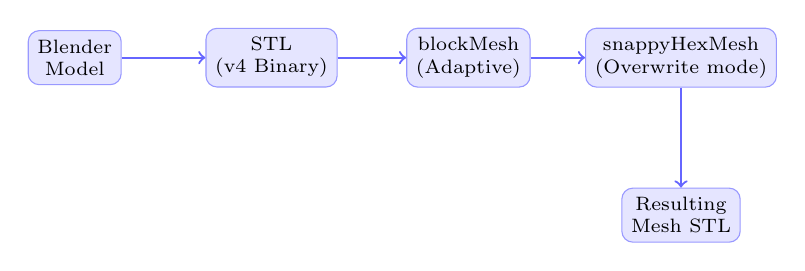
\begin{tikzpicture}[node distance=1.5cm, every node/.style={fill=blue!10, rounded corners, font=\scriptsize, align=center, draw=blue!40}]
            \node (bl) {Blender\\Model};
            \node (stl) [right of=bl, xshift=1cm] {STL\\(v4 Binary)};
            \node (bm) [right of=stl, xshift=1cm] {blockMesh\\(Adaptive)};
            \node (shm) [right of=bm, xshift=1.2cm] {snappyHexMesh\\(Overwrite mode)};
            \node (imp) [below of=shm, yshift=-0.5cm] {Resulting\\Mesh STL};
            
            \draw [->, thick, blue!60] (bl) -- (stl);
            \draw [->, thick, blue!60] (stl) -- (bm);
            \draw [->, thick, blue!60] (bm) -- (shm);
            \draw [->, thick, blue!60] (shm) -- (imp);
        \end{tikzpicture}
    \end{center}
\end{frame}

%% ─────────────────────────────────────────
%% 2. BUG FIX DEEP DIVE
%% ─────────────────────────────────────────
\section{Stability Deep Dive}
\begin{frame}{2.1 The 999\textasciicircum3 Cell Scaling Bug}
    \begin{itemize}
        \item \textbf{Problem}: A baseline logic error caused \texttt{blockMeshDict} to request a background grid of $999 \times 999 \times 999$ cells.
        \item \textbf{Impact}: Instant CPU/RAM exhaustion and system hang during the meshing phase.
        \item \textbf{Technical Fix}:
        \begin{itemize}
            \item Implemented an \textbf{Adaptive Cell-Cap}: \texttt{n\_cells = max(5, min(20, int(1/size)))}.
            \item Capped background mesh to 20 cells while allowing \texttt{snappyHexMesh} to handle local refinements near the STL boundary.
        \end{itemize}
    \end{itemize}
    \begin{center}
        \begin{alertblock}{Scaling Safety}
            This change reduced background memory footprint by 99.9\% while maintaining edge-sharpness via refinement levels.
        \end{alertblock}
    \end{center}
\end{frame}

\begin{frame}{2.2 Context \& IO Robustness (v4)}
    \begin{itemize}
        \item \textbf{Context Fix}: Addon now forces \texttt{bpy.ops.object.mode\_set(mode='OBJECT')} at runtime. 
        \begin{itemize}
            \item Prevents crashes when the "Generate" button is clicked while in \textit{Edit Mode}.
        \end{itemize}
        \item \textbf{Shell Stability}: Switched \texttt{subprocess} execution to a forced \texttt{/bin/bash} environment to ensure OpenFOAM environment variables (sourced via \texttt{source}) persist across commands.
        \item \textbf{IO Verification}: Added \texttt{os.path.isfile()} checks to prevent "Is a directory" errors during mesh re-import.
    \end{itemize}
\end{frame}

\begin{frame}{2.3 Modular Architecture}
    \begin{itemize}
        \item \textbf{\texttt{\_\_init\_\_.py}}: The "DNA" of the addon.
        \begin{itemize}
            \item Manages DNA (Properties), UI Panels (N-panel), and high-level Operators.
            \item Ensures the Blender context is safe before triggering meshing.
        \end{itemize}
        \item \textbf{\texttt{run\_cfmesh.py}}: The OpenFOAM execution engine.
        \begin{itemize}
            \item Handles directory templates, dictionary generation, and subprocess orchestration.
            \item Independent of Blender's UI thread (built for future async support).
        \end{itemize}
    \end{itemize}
\end{frame}

\begin{frame}{2.4 Release History (ZIP Archive)}
    To ensure stability and version-tracking for the FOSSEE team:
    \begin{itemize}
        \item \textbf{v1-v2}: Initial workflow container.
        \item \textbf{v3}: Implemented the \textit{FPE Safety Logic} and forced \texttt{/bin/bash} execution.
        \item \textbf{v4 (Current)}: Added parametric boundary layer controls and \textit{Edit Mode} context stability.
    \end{itemize}
    \begin{center}
        \includegraphics[width=0.8\textwidth]{folder_view.png}
        \caption*{Project Structure \& Versioned Releases}
    \end{center}
\end{frame}

%% ─────────────────────────────────────────
%% 3. ADVANCED CONTROLS
%% ─────────────────────────────────────────
\section{Advanced Controls}
\begin{frame}{3. Parametric Boundary Layers}
    \begin{columns}
    \column{0.5\textwidth}
    The v4 UI introduces direct control over the `addLayers` dictionary:
    \begin{itemize}
        \item \textbf{Final Layer Thickness}: Relative height for viscous sublayer capture.
        \item \textbf{Min Thickness}: Prevents mesh artifacts in sharp V-gaps.
        \item \textbf{Max Medial Ratio}: Automated cessation of layers in narrow channels.
    \end{itemize}
    \column{0.5\textwidth}
    \begin{center}
        \includegraphics[width=0.8\textwidth]{ui_v4_controls.png}
        \caption*{v4 Advanced Sidebar}
    \end{center}
    \end{columns}
\end{frame}

%% ─────────────────────────────────────────
%% 4. RESULTS
%% ─────────────────────────────────────────
\section{Results}
\begin{frame}{4. Mesh Quality \& Validation}
    \begin{itemize}
        \item \textbf{Geometric Precision}: Automatic triangulation enabled before export to ensure STL normal consistency.
        \item \textbf{Quality Metrics}: 0 Non-orthogonality errors verified via \texttt{checkMesh}.
        \item \textbf{Visuality}: Mesh result automatically converted back to STL and imported into Blender workspace.
    \end{itemize}
    \begin{columns}
    \column{0.5\textwidth}
    \begin{center}
        \includegraphics[width=0.9\textwidth]{blender_mesh_wireframe.png}
        \caption*{Imported Hex-Dominant Mesh}
    \end{center}
    \column{0.5\textwidth}
    \begin{center}
        \includegraphics[width=0.9\textwidth]{paraview_clip_layers.png}
        \caption*{Boundary Layer Cross-Section}
    \end{center}
    \end{columns}
\end{frame}

%% ─────────────────────────────────────────
%% 5. CONCLUSION
%% ─────────────────────────────────────────
\section{Next Phase}
\begin{frame}{5. Toward Week 5: Solver Automation}
    \begin{enumerate}
        \item \textbf{Automated Solver Chains}: Direct execution of \texttt{icoFoam} or \texttt{simpleFoam} from the Blender Panel.
        \item \textbf{Async Feedback}: Real-time progress bars to monitor long-running CFD simulations.
        \item \textbf{Data Mapping}: Automated generation of slices and probes for velocity/pressure tracking.
    \end{enumerate}
\end{frame}

\begin{frame}
    \begin{center}
        \Huge \textbf{Thank You!} \\
        \vspace{0.5cm}
        \large Questions?
    \end{center}
\end{frame}

\end{document}
